\documentclass[document.tex]{subfiles}
\begin{document}
\chapter{Wstęp}

\section{Przetwarzanie obrazu i jego rola w automatyce przemysłowej}
	\indent W zagadnieniach technik pomiarowych oraz analizy otoczenia coraz częściej stosowane
	są rozwiązania wykorzystujące systemy wizyjne. Do najpopularniejszych zastosowań przemysłowych wizji maszynowej należą \cite{Machine_Vision_Intro}:
	\begin{itemize}
		\item inspekcja elementów na linii technologicznej
		\item określanie właściwej orientacji i położenia elementów
		\item identyfikacja produktów
		\item pomiary metrologiczne		
	\end{itemize}
	\indent W automatyce przemysłowej gdzie do zagadnień inspekcji
	wcześniej niezbędna była ocena wizualna człowieka, obecnie powszechnie stosuje się systemy wizyjne, 
	w których skład wchodzą kamery przemysłowe, czujniki wyzwalające(np. na bazie pozycji) oraz urządzenie odpowiadającego za proces decyzyjny.
	Występują również rozwiązania w postaci systemów wbudowanych, gdzie inteligentna kamera oprócz
	akwizycji obrazu zajmuje się jego przetwarzaniem i analizą, wykorzystując własny procesor.\cite{Machine_Vision_Intro}\cite{Davies_Machine_Vision}
\\
\begin{center}
	\begin{figure}[h]
	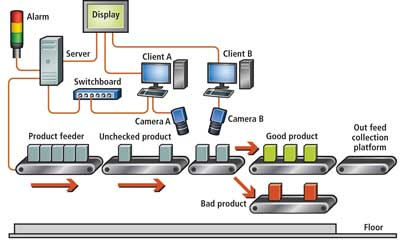
\includegraphics[scale=0.7]{vision_inspection_line}
	\caption{Przykład zautomatyzowanej linii technologicznej wykorzystującej system wizyjny\protect\cite{Vision_systems_article}}
	\label{fig:inspekcja}
	\end{figure}
\end{center}
\clearpage
	\indent Sprawdzanie orientacji i położenia elementów w przemyśle jest wykorzystywane
	między innymi w technologii montażu, gdzie informacje z urządzeń wizyjnych są wykorzystywane
	przez manipulatory przemysłowe do zautomatyzowanego montażu, sortowania oraz paletyzacji wyrobów.\cite{Machine_Vision_Intro}
\\
\begin{center}
	%obrazek - sprawdzanie orientacji
	\begin{figure}[h]
	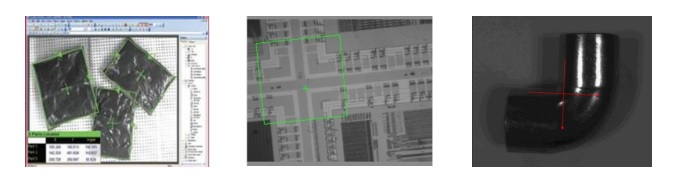
\includegraphics[scale=0.6]{position_orientation_test_images}
	\caption{Przykład obrazów używanych w testowaniu pozycji i orientacji elementów\protect\cite{Machine_Vision_Intro}}
	\label{fig:pozycja_orientacja}
	\end{figure}	
\end{center}
	\indent Identyfikowanie produktów na bazie obrazu cyfrowego jest wykorzystywane przy sortowaniu
	oraz monitorowaniu przepływu elementów i lokalizacji wąskich gardeł.
	Przykładowe metody indentyfikacji to stosowanie kodów kreskowych i kodów DataMatrix.\cite{Machine_Vision_Intro}
\\
\begin{center}
	%identyfikacja
	\begin{figure}[h]
	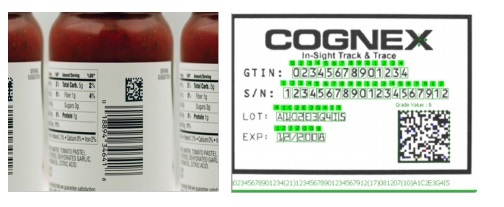
\includegraphics[scale=0.8]{vision_identyfication}
	\caption{Przykład wizyjnej identyfikacji\protect\cite{Machine_Vision_Intro}}
	\label{fig:identyfikacja}
	\end{figure}
\end{center}

\section{Istotność szybkości obliczeń w problemach wizji maszynowej}
%wstęp
\indent Większość praktycznych zastosowań przetwarzania obrazu jako dodatkowej 
informacji w sterowaniu jednym bądź grupą urządzeń, wymaga akwizycji oraz wykonywania
obliczeń w czasie rzeczywistym. Oznacza to, że wybrany algorytm wykorzystywany do 
analizy obrazu cyfrowego, wraz z resztą niezbędnego kodu, musi posiadać czas wykonania 
spełniający narzucone przez sterowany system.

%automatyka przemysłowa
\indent Dla zastosowań przemysłowych. gdzie monitorowane obiekty poruszają się z dużą prędkością, szybkość podjęcia decyzji przez system wizyjny
może być wąskim gardłem dla danej gałęzi linii produkcyjnej. Czas na wykonanie decyzji
(np. o usunięciu wadliwego produktu z przenośnika taśmowego), składa się na czas akwizycji obrazu,
obliczenia sterowania. Standardowe kamery przemysłowe potrafią zrobić nawet powyżej 100 zdjęć na sekundę, a nawet więcej stosując mniejsze rozdzielczości obrazu. Czas przesyłu danych dla
standardu popularnego standardu GigE wynosi maksymalnie 125 MB/s \cite{NI_camera_buses}. Na podstawie tego można stwierdzić, że główny problem będzie stanowił czas obliczenia sterowania i od niego będzie zależeć szybkość działania systemu wizyjnego\cite{Cognex_industrial_cameras}\cite{Basler_industrial_cameras}.

%robotyka mobilna
\indent Inną dziedziną gdzie stosowane jest przetwarzanie obrazu w czasie rzeczywistym
jest robotyka mobilna, gdzie system wizyjny może odpowiadać za:
\begin{itemize}
	\item Sprzężenie niezbędne do obliczenia zmiany położenia i prędkości robota.
	\item Lokalizację przeszkód oraz innych robotów(Swarm Robotics).
	\item Analizę oraz monitorowanie otoczenia.
\end{itemize}
\cite{Mazurek_Robot_Viterbi}\cite{Mobile_Robot_Dumbare}
\\
\indent Podobnie jak dla aplikacji przemysłowych odpowiedzialność za wykorzystanie
pełnych możliwości układów wykonawczych robota jest szybkość obliczania nowych
sterowań. Niezbędne obliczenia mogą być wykonywane bezpośrednio przez urządzenie
sterujące silnikami robota, albo z pomocą osobnej stacji, która połączona zdalnie
z kontrolerem robota jest odpowiedzialna za przeprowadzanie czasochłonnych obliczeń.

\indent Pierwsze rozwiązanie jest korzystne kiedy nie są wymagane duże rozdzielczości obrazu,
skomplikowane i czasochłonne algorytmy przetwarzania obrazu o dużej złożoności obliczeniowej
oraz wysokie prędkości ruchu robota, narzucające krótki czas na obliczenia. 
Stosowane są wtedy najczęściej układy wyposażone mikroprocesory, np. rodzina procesorów ARM oraz x86-64 firmy Intel. Obecne modele są najczęściej wielordzeniowe o taktowaniu nawet powyżej 1GHz
\cite{NXP_ARM} \cite{Intel_Embedded_Processors}.
\\
\begin{center}
	%procesor arm	
	\begin{figure}[h]
	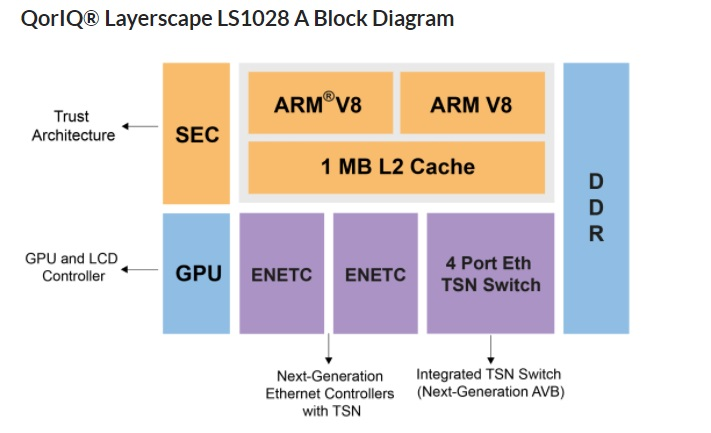
\includegraphics[scale=0.6]{LS1028_arm_design}
	\caption{Procesor \textit{QorlQ Layerscape LS1028} do aplikacji przemysłowych firmy NXP, 
	wyposażony w dwa rdzenie ARMv8\protect\cite{NXP_ARM}}
	\label{fig:arm_processor}
	\end{figure}
\end{center}	
Dla rozwiązań bardziej wymagających pod względem szybkości obliczeń stosowane są układy
FPGA, w których logika przetwarzania informacji obrazu jest zaprojektowania w języku
HDL(VHDL, Verilog). Zapewniają one najszybsze prędkości obliczeń ze względu na sprzętową implementację algorytmów. \cite{FPGA_Design}\cite{VHDL_FPGA}. 
\indent Drugie rozwiązanie gdzie osobne urządzenie jest używane do przetwarzania obrazu, umożliwia użycie mniej kosztownego procesora po stronie robota. Wystarczające do sterowania silnikami jest zastosowanie układu wykorzystującego mikrokontroler(np. z rodziny STM32 bądź Atmel AVR)\cite{STM32_microcontrollers} \cite{Atmel_microcontrollers}. 
\\
\begin{center}
%stm32 microcontroller
	\begin{figure}[h]
	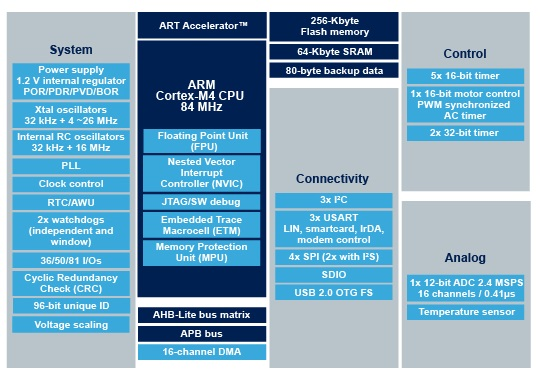
\includegraphics[scale=0.8]{stm32_design}
	\caption{Structura mikrokontrolera \textit{STM32F401CC}\protect\cite{STM32_microcontrollers}}
	\label{fig:stm32}
	\end{figure}
\end{center}
Zewnętrzna jednostka obliczeniowa pozwala na wykorzystanie możliwości konwencjonalnych wielordzeniowych procesorów dla komputerów PC oraz procesora karty graficznej, który jest wyspecjalizowany w obliczeniach równoległych\cite{GPU_vs_CPU_nvidia} \cite{Computer_Architecture_Patterson_Hennesy}\cite{GPUs_Closer_Look}. 
Dzięki kombinacji CPU i GPU możliwe jest przyspieszenie operacji,
które mogą być wykonywane równolegle oraz rozdzielenie obciążenia obliczeniowego pomiędzy
procesor i kartę graficzną. \\
%podsumowanie
\indent Podsumowując, szybkość obliczeń systemu wizyjnego w robotyce mobilnej decyduje o tym jakie
mogą być maksymalne parametry ruchu robota - prędkość, przyspieszenie, ilości robotów współpracujących w zagadnieniach robotyki roju(Swarm Robotics) oraz poziomie skomplikowania
analizy obrazu. W przypadku problemów wizji maszynowej dla zastosowań przemysłowych czas poświęcony na analizę każdego zdjęcia ma wpływ na szybkość działania całej linii produkcyjnej, co ma bezpośredni wpływ na wydajność i koszty produkcji.  

\section{Cel, zakres i zastosowania pracy}
\indent Celem pracy jest implementacja algorytmu Viterbiego w celu wykrywania linii na zaszumionym obrazie cyfrowym oraz analiza porównawcza dla rożnych wersji napisanego algorytmu.
Rozpatrywana będzie implementacja szeregowa i równoległa dla CPU w języku C++ oraz 
napisana pod procesor karty graficznej z wykorzystaniem biblioteki OpenCL. Implementacja
z wykorzystaniem biblioteki OpenCL będzie składała się z dwóch wariantów:
\begin{itemize}
	\item całkowicie wykonywany przez GPU
	\item hybrydowy - podział obciążenia obliczeniowego pomiędzy procesor i kartę graficzną.
\end{itemize} 
Następnie dla różnych konfiguracji sprzętowych zostanie zrobione porównanie ich szybkości.
Na podstawie powyższej analizy zostanie wybrany najlepszy wariant realizacji 
algorytmu Viterbiego, co będzie mogło być później zastosowane w sterowaniu ruchem robota
mobilnego.  

\end{document}